%This work is licensed under the Creative Commons License Attribution 4.0 International (CC-BY 4.0) 
%https://creativecommons.org/licenses/by/4.0/legalcode 
\documentclass[rgb]{standalone}
\usepackage{tkz-euclide}
\begin{document}
	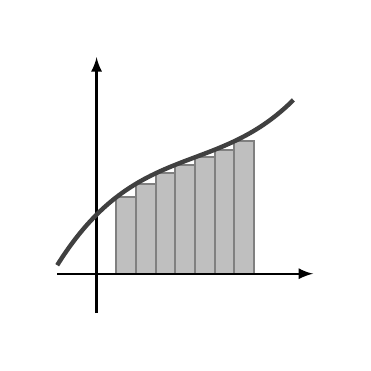
\begin{tikzpicture}[scale=0.5, font=\Large]
		\draw[draw=none] (-1.75,-1.75) -- (-1.75,6.25) -- (6.25,6.25) -- (6.25,-1.75) -- cycle;
		\foreach \x in {0.5,1,...,3.5} 
		{
			\draw[thick, gray,fill=gray, fill opacity=0.5, domain=1.5:3.5, smooth,variable=\x]  (\x,0) -- (\x, {1.5+\x-0.25*\x*\x+1/30*\x*\x*\x}) -- (\x+0.5,{1.5+\x-0.25*\x*\x+1/30*\x*\x*\x}) -- (\x+0.5,0);
		}
		\draw[thick, -latex] (-1,0) -- (5.5,0);
		\draw[thick, -latex] (0,-1) -- (0,5.5);
		\draw[ultra thick,domain=-1:5, smooth, samples=300, variable=\x, darkgray] plot (\x, {1.5+\x-0.25*\x*\x+1/30*\x*\x*\x});
	\end{tikzpicture}
\end{document}